%%%%%%%%%%%%%%%%%%%%%%%%%%%%%%%%%%%
% PART II: Experiment definition module
%%%%%%%%%%%%%%%%%%%%%%%%%%%%%%%%%%%

\part{The Abstract Experiment Definition Language -- AEDL}

\chapter{General Concept}

The aim of AEDL is to describe a large variety of complex experiments
by a limited number of parameters and to allow a representation of
very different setups within one data structure, thus enabling a
universal rate and $\chi^2$ computation. Usually in dealing with
experiment simulations a new piece of code is written and compiled
for each different experiments. In many cases even changes of some
parameter like the number of bins requires the recompilation of
large portions of the source code. This technique may however soon
reach its limits in cases where the simulated experiments are rather complex
and/or more than one kind of experiment is going to examined. Furthermore
is is very difficult to assure the correctness of the results obtained
in this way since every time a new piece of code is added to handle a new
experiment new errors will be introduced.

Thus a general and flexible experiment description language is needed. 
A neutrino experiment can be split into three parts: source, oscillation
and detection. The sources within \GLOBES\ are assumed to be stationary
point sources and each experiment has only one source. Specifically this
does not allow to study cases where the time dependence of the neutrino flux
is of physical significance like \eg\ in supernov\ae. It however is possible
to study beams which have a bunch structure, since the time dependence of the
neutrino source is physically only in as far important as it is used to
suppress backgrounds. Also geometrical effects of a source distribution like
\eg\ in the Sun can not described in this way. For this kind of sources
the oscillation part of an 
experiment is simply
given by the baseline and the matter density profile. 


While
it is comparatively simple to define a general neutrino source 
and the oscillation physics, the general properties of a detector are more
complicated. The basic assumption in building an abstract detector description
is \emph{linearity}, \ie\ two neutrino events do not interfere with each other.
Furthermore it is assumed that all information on the oscillation physics 
is given by the \emph{reconstructed} flavour and energy of a 
neutrino event. The term ``reconstructed'' implies that there is not a single
well defined value for each event and variable but a distribution of possible
values. This illustrated in figure~\ref{fig:distro} for the energy variable.
The same is of course possible with the flavour variable. In that case however
only discrete values are possible.
%
\begin{figure}[h!]
\begin{center}
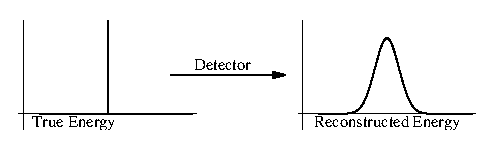
\includegraphics[width=0.6\textwidth]{mapping}
\end{center}
\caption{\label{fig:distro} A detector maps the true values into
a distribution of reconstructed values of a parameter. Here the energy is 
shown.}
\end{figure}
% 

This picture also can be formulated in a more mathematical language. Let $x$
be the true variable and $x'$ the reconstructed variable then $f(x)$ is the
distribution of true values and $p(x')$ is the distribution of reconstructed
values. Then the detector function  $D(x,x')$ which describes 
the mapping performed by the detector is defined by
\begin{eqnarray}
\label{eq:mapping}
p(x')&=&\int dx\, f(x)\cdot D(x,x')\,.
\end{eqnarray}
Obviously equation~\ref{eq:mapping} can only describe the detector correctly
when the condition of linearity is fulfilled. Within this model a detector
is completely specified by a set of $D(E,E')$ for the energy variable $E$
and a set $D(F,F')$ for the flavour variable $F$, where usually $D(E,E')$ also
depends on the true flavour $F$ as well as $D(F,F')$ depends on the true energy
$E$. Those sets of mapping functions usually will be obtained by a 
full detector simulation and can be obtained by using as input 
distribution $f(x)$ a delta distribution $\delta(x-x_0)$.

In order to allow a systematic experiment definition including various
sources of systematical errors we use several layers. The first layer is
the so called ``channel'', it is the link between the oscillation physics
and the detector. A channel specifies how a certain neutrino type in the 
source is mapped into a reconstructed neutrino type, \eg\ a muon neutrino
oscillates into an electron neutrino and subsequently interacts via
quasi-elastic charged current scattering. The measured energy and direction of
the electron in the detector finally allow to reconstruct the neutrino energy.
The channels are the building blocks for so called ``rules'' which
contain information like the efficiencies and systematical errors. An example
could look like this: the efficiency for quasi-elastics electron neutrino
events is $0.4$. There is a fraction of $0.01$ of all neutral current events
which are mis-identified as quasi-elastic electron neutrino events. 
The neutral current fraction is only known within $10\%$ and there is
an energy scale uncertainty of $100\,\mathrm{MeV}$. Thus a rule connects the
event rates to the calculation of a $\chi^2$ which properly includes 
systematical errors. This $\chi^2$ is then the starting point for the
oscillation physics analysis.

%%%%%%%%%%%%%%%%%%%%%%%%%%%%%%%%%%%%%%%%%%%%%%%%%%%%%%%%%%%%%%%%%%%%%%%%%%%
\chapter{Getting started}

As a first example we discuss how to define a neutrino factory experiment using
AEDL. The first line of every experiment definition file is
\begin{quote}
{\tt !\%GLoBES}
\end{quote}

We tell \GLOBES\ that we want to use the built-in neutrino factory
flux, by setting the beam type variable to $1$. The target mass 
is $50\,\mathrm{kt}$ and a total of $ 4.264\cdot10^{21}$
muons is stored. The data is divided into 20 energy bins ranging from
$4\,\mathrm{GeV}$ to $50\,\mathrm{GeV}$. 
\begin{quote}
{\tt /* beam */}\\
{\tt \$beam\_type = 1}\\
{\tt \$target\_mass = 50}\\
{\tt \$stored\_muons = 4.264e+21}\\
{\tt \$numofbins = 20}\\
{\tt \$emin = 4.0}\\
{\tt \$emax = 50.0}
\end{quote}

Next a file has to be specified which contains the cross section we want to 
use.
\begin{quote}
{\tt /* cross section */}\\
{\tt cross(\#CC)<}\\
{\tt \hspace*{3ex}@cross\_file = XCC.dat}\\
{\tt >}
\end{quote}
The command {\tt cross} tells the parser that a cross section environment
begins and has the name {\tt \#CC}. These names are used to refer later on
to this specific environment and each name begins with a leading {\tt \#}.
Whenever we need to specify a cross section from here on we can use {\tt \#CC}
to refer to the cross section as given in the file {\tt XCC.dat}.


Of course also the baseline and matter profile have to be specified, which
 looks like this
\begin{quote}
{\tt /* baseline */}\\
{\tt \$baseline = 3000.0}\\
{\tt \$densitytab = \{3.5\}}\\
{\tt \$lengthtab = \{3000.0\}}\\
{\tt \$density\_error = 0.05}
\end{quote}
The curly brackets used for the definition of {\tt \$densitytab} and
{\tt \$lengthtab} delimit as simple list of numbers -- here the lists
have length $1$. {\tt \$density\_error} is the relative $1\,\sigma$ uncertainty
on the density.

The energy resolution function can easily be specified with
\begin{quote}
{\tt /* energy resolution */}\\
{\tt energy(\#MINOS)<}\\
{\tt \hspace*{3ex}@algorithm = 1}\\
{\tt \hspace*{3ex}@bins = 20}\\
{\tt \hspace*{3ex}@emin = 4.0}\\
{\tt \hspace*{3ex}@emax = 50.0}\\
{\tt \hspace*{3ex}@energy\_resolution = \{0.15,0.0,0.0\}}\\
{\tt >}
\end{quote}
The {\tt energy} command opens the corresponding energy environment and
the energy resolution function defined here is refered to by the name 
{\tt \#MINOS}. Out of several possibilities it employs algorithm $1$,
the simplest and fastest one. The actual energy resolution is specified
by the energy resolution variable which is a list of three elements. Each 
element is one parameter of a general resolution function as defined in 
equation ~\ref{eq:sigma_e}.

Now we define the one appearance and the corresponding disappearance 
channel of a neutrino factory: 
$\nu_e\rightarrow\nu_\mu$  and $\bar\nu_\mu\rightarrow\bar\nu_\mu$ 
($\mu^+$ stored).
\begin{quote}
{\tt /* channels */}\\
{\tt channel(\#appearance)<}\\
{\tt \hspace*{3ex}@channel = +: +: electron: muon: \#CC: \#MINOS}\\
{\tt >}\\
{\tt channel(\#disappearance)<}\\
{\tt \hspace*{3ex}@channel = +: -: muon: muon: \#CC: \#MINOS}\\
{\tt >}
\end{quote}
The first $\pm$ selects the polarity, \ie\ wether $\mu^+$ or $\mu^-$ are 
stored. The second $\pm$ determines whether neutrinos or anti-neutrinos are
taken from the flux table. The third position defines the initial flavour
and the forth position the final flavour, followed by the name of the cross
section and energy resolution function.

The last step is to assemble the channels into a rule.
\begin{quote}
{\tt /* rules */}\\
{\tt rule(\#rule1)<}\\
{\tt \hspace*{3ex}@signal = 0.45 @ \#appearance}\\
{\tt \hspace*{3ex}@signalerror = 0.001 : 0.0001}\\
{\tt \hspace*{3ex}@background = 1.0e-05 @ \#disappearance}\\
{\tt \hspace*{3ex}@backgroundcenter = 1 : 0.0}\\
{\tt \hspace*{3ex}@backgrounderror = 0.05 : 0.0001}\\
{\tt \hspace*{3ex}@errordim = 0}\\
{\tt \hspace*{3ex}@energy\_window = 4.0 : 50.0}\\
{\tt >}
\end{quote}
The signal variable says that the signal in our experiment is the 
channel named {\tt \#appearance} with an constant efficiency of $0.45$.
The signal error variable has two components: the first one is the
normalization error of the signal, here it is $0.1\%$. The second component
signifies the energy calibration error of the signal, whose definition 
can be found in section~\ref{sec:energy}. The background variable
specifies the composition of the beam background and this case is
given by the channel named {\tt \#disappearance}, \ie\ this are
the muons whose charge has been mis-identified. They enter the calculation
with an efficiency of $1\cdot 10^{-5}$. The background center variable allows
to rescale the total background contribution which is especially useful if
there are many background components. 
The background error variable is defined in the same way as the signal error
variable, \ie\ we have a $5\%$ background uncertainty.
The error dimension variable selects how
the systematical errors are treated according to table~\ref{tab:error_dim}. 


The above defined experiment represents a first version of a neutrino factory
experiment. It still lacks the correct energy dependence of the efficiencies
and of course the channels and rules for the operation with $\mu^-$ stored

%%%%%%%%%%%%%%%%%%%%%%%%%%%%%%%%%%%%%%%%%%%%%%%%%%%%%%%%%%%%%%%%%%%%%%%
\chapter{Features of the  AEDL}

%%%%%%%%%%%%%%%%%%%%%%%%%%%%%%%%%%%%%%%%%%%%%%%%%%%%%%%%%%%%%%%%%%%%%%%%
\section{Source properties}
\label{sec:source}

\GLOBES\ handles only point sources, thus it is not possible
to study effects from the finite size of the neutrino production
region like in the Sun. Furthermore only one source for each experiment
is possible, this make it impossible\footnote{at least rather tricky} 
to simulate multiple source experiments like KamLAND. All neutrino
sources usable within \GLOBES\ therefore can be specified by the
flux spectra for each flavour and CP sign and the total luminosity
of the source. There are two principal ways to provide a flux:
use a built-in source or a file provided by the user. 

The built-in source is muon decay, since the neutrino
spectra and flavour composition are known analytically in that case. For 
this sources the energy of the parent particle has to be specified
and the number of useful decays per year.

In the latter case the fluxes are read from a file with seven rows and
501 lines.
\begin{quotation}
$ E\quad
\Phi_{\nu_e}\quad
\Phi_{\nu_\mu}\quad
\Phi_{\nu_\tau}\quad
\Phi_{\bar\nu_e}\quad
\Phi_{\bar\nu_\mu}\quad
\Phi_{\bar\nu_\tau}$
\end{quotation}
where the energy values are evenly spaced. 
For accessing fluxes at 
arbitrary energies linear interpolation is used. Once the energy leaves the
range of values given in the file $0.0$ is returned. The units used for the
fluxes are not specified and right now each flux has its own fudge factor
which is hard encoded in the file {\tt nufact.c}. The problem is that
in computing the normalization one has to know things like number of target
particles per unit mass asf. which is not always straightforward. Thus a fudge
factor will be useful in any case. Right now however this is not the only 
fudge factor since for some experiments the definition of their target mass
involves another fudge factor. 

Since many sources have two modes of operation, it is possible to define
a pair of fluxes by using the polarity flag when loading the files. Usually
files connected in this way use the suffixes ``plus'' and ``minus'' in the 
file names. The individual members of the pair can be accessed by the polarity
variable. Also the built-in fluxes provide this choice.


For sources based on $\pi$-decay and nuclear reactors the total power
involved defines how many neutrinos are produced therefore this variable is
used to define the luminosity. Furthermore it is useful to define 
the operation time of an experiment in years. Note however that the 
number of events used in analysis only depends on the product of
\begin{equation}
\mathrm{mass}\,\left[10^6\,\mathrm{kg}\right]\times \mathrm{time}
\,\left[\mathrm{years}\right]\times\left\{ \begin{array}{c}
\mathrm{source~power}\,\left[\mathrm{MWy}\right]\\
\mathrm{useful~decays}\,\left[\mathrm{year}^{-1}\right]
\end{array}\right.\,.
\end{equation}
%%%%%%%%%%%%%%%%%%%%%%%%%%%%%%%%%%%%%%%%%%%%%%%%%%%%%%%%%%%%%%%%%%%%%
\section{Oscillation properties}



\subsection{Baseline \& matter profile}
The purpose of this module is to specify the path the neutrinos
are traveling. The central piece of information is the total length
of the path - the baseline\index{Baseline}
\begin{equation}
L\,\left[\mathrm{km}\right]
\end{equation} 

Furthermore there is
the matter profile encountered along the baseline which can be set in
several ways. The simplest way is to use a constant density corresponding
to the average density along the baseline calculated using the 
PREM\cite{Stacey} onion shell model of the 
Earth\index{PREM}\index{Earth matter density}.

Another possibility is to use several layers of constant density each in 
order to improve the approximation to the actual Earth matter profile. In this
case the user specifies the total baseline and the number of layers. The
time consumed in computing the oscillation probabilities is directly 
proportional to the number of layers.

The third possibility to specify the matter profile is to provide a list
of thicknesses and densities for the layers. 

For any type of profile a central value $a$ and a corresponding error 
$\delta a$ have to be specified\index{Density error}\index{Density center}.
\begin{equation}
\label{eq:density_error}
\rho(x)=a\cdot\rho_0(x)\,\left[\frac{\mathrm{g}}{\mathrm{cm}^2}\right]\,
\end{equation}
where $\rho_0(x)$ is the matter profile as chosen by the user and $\rho(x)$ is
the one used in the calculation of the oscillation probabilities. The default
value for $a$ is $1$ and a typical value for $\delta a = 0.05$. 


%%%%%%%%%%%%%%%%%%%%%%%%%%%%%%%%%%%%%%%%%%%%%%%%%%%%%%%%%%%%%%%%%%%%%%%%%%%%%
\section{Detection properties}

The most obvious property of the neutrino detection is the total
active mass of the target as already defined in section~\ref{sec:source}.

\subsection{Cross section}
\label{sec:cross_section}

Cross sections\index{Cross sections} are used as part of the 
channel definition 
(see section~\ref{sec:channel}) and have to be provided by the user in form
of a file. Cross section are in general given as differential cross section
divided by the energy
\begin{equation}
\hat\sigma(E)=\sigma(E)/E\,\left[ 10^{-38}\,
\frac{\mathrm{cm}^2}{\mathrm{GeV}^2} \right]
\end{equation}
The cross section files have seven rows and $1001$ lines.
\begin{quotation}
$log_{10} E\quad
\hat\sigma_{\nu_e}\quad
\hat\sigma_{\nu_\mu}\quad
\hat\sigma_{\nu_\tau}\quad
\hat\sigma_{\bar\nu_e}\quad
\hat\sigma_{\bar\nu_\mu}\quad
\hat\sigma_{\bar\nu_\tau}$
\end{quotation}
where the logarithm of the energy values is evenly spaced. 
For accessing cross section at 
arbitrary energies linear interpolation is used. Once the energy leaves the
range of values given in the file $0.0$ is returned.


\subsection{Channels}
\label{sec:channel}

Channels\index{Channel} represent an intermediate level in between 
the pure oscillation 
physics given by the oscillation probability $P_{\alpha\beta}$ and the
detected signal and background. A channel basically describes the path from one
initial state in the source to one interaction type (IT) in  the detector.  
Therefore a channel consists of the description of the initial state given 
by the polarity 
of the source, \eg\ muons or anti-muons in a neutrino factory, by the CP 
eigenvalue of the initial state, \ie\ neutrino or anti-neutrino and by the 
initial flavour. A channel furthermore consists of the interaction type in the
detector given by the final flavour of the neutrino, the interaction cross
section and the energy resolution function. 
 
For the calculation of event rates, the first step is to compute the number of
events for each IT in the fiducial mass of the detector for each 
neutrino flavor and energy bin. The second step is to include the detector 
effects coming from
the insufficient knowledge used in the event reconstruction. We combine these
two steps in order to obtain the differential event rate spectrum for each
flavor and IT as seen by the detector, which we call a ``channel''. 
The master formula for the differential event rate for each channel 
is given by
%%%%%%%%%%%%%%%%%%%%%%%%%%%%%%%%%%%
\begin{eqnarray}
\label{eq:master_event}
\frac{dn_{\beta}^{\text{IT}}}{dE'}=&&N\,\int \int dE\,d\hat{E}\quad
\underbrace{\Phi_{\alpha} (E)}_{\mathrm{Production}} \times \nonumber\\
&&\underbrace{\frac{1}{L^2} P_{(\alpha\rightarrow\beta)}(E,L,\rho;\theta_{23},
\theta_{12},\theta_{13},
\Delta m^2_{31},\Delta m^2_{21},\deltacp)}_{\mathrm{Propagation}}
\times \nonumber \\ &&\underbrace{\sigma^{\text{IT}}_f(E)
k_f^{\text{IT}}(E-\hat{E})}_{\mathrm{Interaction}} \times \nonumber \\
&&\underbrace{ T_f(\hat{E}) V_f(\hat{E}-E')}_{\mathrm{Detection}}\,,
\end{eqnarray}
%%%%%%%%%%%%%%%%%%%%%%%%%%%%%%%%%%%
where $\alpha$ is the initial flavor of the neutrino and 
$\beta$ is the final flavour, 
$E$ is the incident neutrino energy, $\Phi_{\alpha} (E)$ is the flux of the 
initial flavor at the
source, $L$ is the baseline length, $N$ is a normalization factor, and 
$\rho$ is the matter density. The interaction term is composed of 
two factors, which are the total cross section 
$\sigma^{\text{IT}}_\beta(E)$ for the flavor $f$ and
the interaction type IT, and the energy distribution of the 
secondary particle $k_\beta^{\text{IT}}(E-\hat{E})$ with 
$\hat{E}$ the energy of the secondary particle. The detector properties are 
modeled by the threshold function $T_\beta(\hat{E})$, coming from the the 
limited resolution or the cuts in the analysis, and the energy resolution 
function $V_\beta(\hat{E}-E')$ of the secondary particle. Thus, $E'$ is the 
{\em reconstructed} neutrino energy.

Since it is rather cumbersome to numerically solve this double integral,
we split the two integrations. We first evaluate the integral over
$\hat{E}$, where the only terms containing $\hat{E}$ are
$k_\beta^{\text{IT}}(E-\hat{E})$,  $ T_\beta(\hat{E})$, and 
$ V_\beta(\hat{E}-E')$, and define:
\begin{eqnarray}
\label{eq:e_res} 
R_\beta^{\text{IT}}(E,E')\,\epsilon_\beta^{\text{IT}}(E')
 \equiv
\int d\hat{E} \quad T_\beta(\hat{E})\,k_\beta^{\text{IT}}(E-\hat{E})
\,V_\beta(\hat{E}-E')\,, 
\end{eqnarray}

!!!!!!!!!!!!
Do we need $\epsilon(E')$ ???
!!!!!!!!!!!!

Thus $R_\beta^{\text{IT}}(E,E')$ describes the energy response of 
the detector, \ie\ a neutrino with a (true) energy of $E$ has a probability
of $R_\beta^{\text{IT}}(E,E') dE'$ to have a reconstructed energy 
in between $E'$ and $E'+dE'$. The function $R(E,E')$ is also refered to
as energy resolution function or smearing matrix in its actual representation
in the program\index{Energy resolution}\index{Smear matrix}. The detailed
definition and initialization of the energy resolution function is described
in section~\ref{sec:energy}.

\subsection{Rules}
\label{sec:rules}

The set of rules\index{Rule} for an experiment is the final 
link between the event rate
computation and the statistical analysis. The information given by the rules
specifies how the $\chi^2$ is computed based on the raw event rates as 
described by the channels including possible systematical errors. 
Therefore a rule has two parts: the first part describes how signal and 
background events are composed out of the channels and the second part
specifies which systematical errors are considered and what the size
of the relevant errors is.

Based on the definition of channels it is possible to assemble the 
signal and background event numbers for each bin.  
The number of events in one channel and  in one bin\index{Bin} $i$ is given by
\begin{equation}
n_i^c=\int_{E_i-\Delta E/2}^{E_i+\Delta E/2} dE' \quad
\frac{dn_{\beta}^{\text{IT}}}{dE'} (E')
\end{equation}
where $c$ is the channel index.
Note that the events are binned according to their \emph{reconstructed} energy.
The signal $s_i$ in one bin for a rule now can be composed out of 
several channels by
\begin{equation}
s_i=\epsilon_{c_1}\cdot n_i^{c_1}\,+\,\epsilon_{c_2}\cdot n_i^{c_2}\,+\,\ldots
\end{equation}
where the $\epsilon$'s are weight factors determined by the properties
of the detector.
Similarly the background in one bin $i$ can be specified by
\begin{equation}
b_i=\epsilon_{c_1}\cdot n_i^{c_1}\,+\,\epsilon_{c_2}\cdot n_i^{c_2}\,+\,\ldots
\end{equation}
Quite often it is not sufficient to have constant efficiencies and therefore
it is possible to define efficiencies for each bin and channel $\alpha_i^c$
and thus the event rates in one bin become
\begin{equation}
s_i=\epsilon_{c_1}\alpha_i^{c_1}\cdot n_i^{c_1}\,+
\,\epsilon_{c_2}\alpha_i^{c_2}\cdot n_i^{c_2}\,+\,\ldots\,,
\end{equation}
and analogous for $b_i$.



The set of all $s_i$'s and $b_i$'s now can be composed in a form that takes
some types of systematical error into account. The two most important and
most easily parameterized systematics are a normalization and an energy
calibration error. These error are considered separately for the signal events
and the background events. The implementation of the normalization error
is straight forward
\begin{equation}
s_i(a):=a\cdot s_i
\end{equation} 
with an analogous definition for the background events.

For the parameterization of an energy calibration error two possibilities
are implemented. The first one being somewhat simpler, whereas the second one
is more accurate but requires a careful choice of parameters. The first 
option is
\begin{equation}
s_i(a,b):=s_i(a)+b\cdot s_i\, E_i/(E_\mathrm{max}-E_\mathrm{min})
\end{equation}
and it is refered to as tilt since it describes a linear distortion, a tilt
of the event rate spectrum. The second option is closer to an actual energy
calibration error, which basically amounts to replacing the reconstructed 
energy $E'$ by $(1+b)\cdot E'$ and we use following approximation
\begin{eqnarray}
s_i(b)&=& (1+b)\cdot(s_{k+1}-s_k)\cdot\delta+s_i\,,\\
\delta&=&b\cdot(i+\Delta E+ 1/2)+i\,,\nonumber\\
k&=&\mod(\delta,1)\,.\nonumber
\end{eqnarray}
Special care is required at the boundaries when $k<1$ or $k+1>N_\mathrm{bins}$,
since there $s_k$ or $s_{k+1}$ may not have been calculated. One possibility
to deal with those cases is to assume that for those values of $k$ $s_k$ is
zero. This is the default. In cases where $s$ at the boundary is however still
sizeable this may lead to intolerable errors and subsequently to a wrong
estimate of the impact of a calibration error. Therefore in those cases it
is advisable to truncate the analysis range by a few bins at the boundary
and therefore ensure in this way that only those $s_i$ are used whose index
$k$ is within the range $1,\ldots, N_\mathrm{bins}-1$. 

In order to perform this fine tuning, it is possible to constrain 
the energy range from which the data are taken for the 
analysis\index{Energy window}. This is achieved by setting the energy window
variable. The purpose is mainly to allow a fine tuning of the description
of an energy calibration error. The default setting is that the energy window
coincides with the range defined by the minimal and maximal reconstructed 
energy. For the error dimension using the calibration method (C) it is 
advisable to reduce the energy window by two or three bins at both the lower
and upper end. As a rule of
thumb consider the three standard deviations error on the calibration and
evaluate the corresponding shift in $E'$ at the lower and upper energy limit 
and reduce the analysis range by this amount.

Thus the total event rate $x_i$ in a bin $i$ is given by
\begin{equation}
x_i(a,b,c,d)=s_i(a,b)+b_i(c,d)
\end{equation}
and thus a function of four parameters. The central values for all of
the four parameters are always needed. They are called signal normalization
($a$), signal tilt/calibration ($b$), background  normalization ($c$) and
background tilt/calibration ($d$). The default values are
\begin{equation}
a=1\,,\quad b=0\,,\quad c={\tt NaN}\,,\quad d=0\,,
\end{equation}
thus for the background normalization $c$ a value has to be specified in 
\emph{all} cases.

The four parameters $a,b,c,d$ have been introduced in order to describe
systematical uncertainties, they are so called nuisance parameters.
For the analysis of the systematical errors the so called 
 pull method is 
used~\cite{Fogli:2002pt}\footnote{In fact the pull method
was employed already in~\cite{Huber:2002mx} before 
\cite{Fogli:2002pt} appeared.}. 
In the  pull method $k$ systematical errors are included by introducing 
$k$ additional variables $\zeta_k$, which will  be called 
nuisance parameters in the following. 
The nuisance parameters describe the dependence of the event rates on the 
various sources of systematical errors, \eg\ an error on the total 
normalization is included by multiplying the expected number of events in 
each bin by a factor $(1+\zeta_1)$. The variation of $\zeta_1$ in the fit 
is constrained by adding a penalty $p_1$ to the $\chi^2$-function. In case 
of a  Gau\ss ian distributed systematical error this penalty is 
given by
\begin{equation}
\label{eq:penalty}
p_i=\frac{(\zeta_i-\zeta_i^0)^2}{\sigma_{\zeta_i}^2}\,,
\end{equation}
where $\zeta_i^0$ denotes the mean and $\sigma_{\zeta_i}$ the standard 
deviation of the corresponding nuisance parameter, \ie\ the amount of 
systematical uncertainty. 
The resulting $\chi^2$ is then minimized with respect to all nuisance 
parameters $\zeta_i$ and this yields $\chi^2_\mathrm{pull}$
\begin{equation}
\chi^2_\mathrm{pull}(\boldsymbol{\lambda}):=\min_{\{\zeta_i\} } \,\, \left( 
\chi^2(\boldsymbol{\lambda},
\zeta_1, \ldots, \zeta_k)+ \sum_{j=1}^{k} p_j(\zeta_j)\right)\,,
\end{equation}
where $\boldsymbol{\lambda}$ denotes the oscillation parameters 
including the matter density
$\rho$. One advantage of the pull method is that whenever the number $N$ of 
data points is much larger than $k$, it is numerically easier to compute 
$\chi^2_\mathrm{pull}$ than to invert the $N\times N$ covariance matrix. For
the experiments considered here $N$ is typically $20$ and $k\sim 4$, thus
the pull method is numerically much faster. Moreover it is more flexible and 
allows the inclusion of systematical errors also for a 
Poissonian $\chi^2$-function.
In~\cite{Fogli:2002pt} it was shown that the pull method and the covariance
based approach are equivalent for a Gau\ss ian and linear model. In general
there is a separate $(\chi^2_\mathrm{pull})^\alpha$ for each rule $\alpha$, 
\ie\ pair of signal and background spectra, with a separate set of 
nuisance parameters $\zeta_i^\alpha$. In this case $\chi^2_\mathrm{pull}$
is the sum of all individual  $(\chi^2_\mathrm{pull})^\alpha$.
In this way the dependence on the $k$ nuisance parameters has been eliminated 
from $\chi^2_\mathrm{pull}$. 

The user has the possibility to choose the set $\{\zeta_i\}$ of nuisance 
parameters which are marginalized. This achieved with the error dimension 
variable\index{Error dimension}, and the different possibilities are shown in
table~\ref{tab:error_dim}. If a parameter is designated with $+$, it will
be marginalized and therefore the corresponding error needs to have a non-zero
value. In the cases labeled (number 4 and 8) ``total rates'' 
the summation over the bins is performed \emph{before} computing 
the $\chi^2$. The case labeled (number 7) ``spectrum only'' leaves the 
normalization free ($\sigma_a=\sigma_c=\infty$) and therefore counts only the 
spectral information in the data. As a consequence
the settings for the normalization error will be ignored. It is furthermore
possible to extend the set of error dimensions and thus the set of possible 
systematical errors to be studied, but this requires proper C programing, 
compiling and linking with \GLOBES. The interface for user defined error 
dimensions is described in detail in section~\ref{sec:ud_error_dim}.

%%%%%%%%%%%%%%%%%%%%%%%%%%%%%%%%%%%%%%%%%%%%%%%%%%%%%%%%%%%
\begin{center}
\begin{table}[hbt!]
\begin{center}
\begin{tabular}[h]{|c|cccc|c|c|}
\hline
Error dimension&$a$&$b$&$c$&$d$&Tilt/Calibration&Remarks\\
\hline
\hline
0&+&+&+&+&T&\\
2&-&-&-&-&-&\\
4&+&+&+&+&T&total rates\\
7&o&-&o&-&-&spectrum only\\
8&-&-&-&-&-&total rates\\
9&+&+&+&+&C&\\
\hline
\end{tabular}
\caption[Table of error dimensions]{\label{tab:error_dim}
Values of the error dimension variable and their meaning.
 }
\end{center} 
\end{table} 
\end{center}
%%%%%%%%%%%%%%%%%%%%%%%%%%%%%%%%%%%%%%%%%%%%%%%%%%%%%%%%%%%%%%



%%%%%%%%%%%%%%%%%%%%%%%%%%%%%%%%%%%%%%%%%%%%%%%%%%%%%%%
\subsection{Energy resolution function}
\label{sec:energy}

The origin and meaning of the energy resolution function 
$R^c(E,E')$ was already discussed in 
section~\ref{sec:channel} and  a mathematical definition
was given in equation~\ref{eq:e_res}. Here we deal with
how to tell \GLOBES\ which energy resolution function it should
use. This also naturally involves the issue how the actual convolution
of the differential event rate spectrum with $R_\beta^{\text{IT}}(E,E')$
is performed. First we will discuss the mathematical structure of
the problem and then the various algorithms and possibilities which
\GLOBES\ offers are introduced. 


Before going into the details we define that the range from $E_\mathrm{min}$
to $E_\mathrm{max}$ is divided in a certain number of bins $N_\mathrm{bins}$.
These bins form a partition, which not necessarily is equidistant. The 
partition is any case completely defined by specifying $E_\mathrm{min}$
and $E_\mathrm{max}$ and the size of each bin  $\Delta E_i$. It is also
straightforward to compute the midpoint of each bin $E_i$.
In order to obtain the number of events 
$n_i^c$ from one channel $c$ in one bin $i$ one has to solve this integral
%
\begin{eqnarray}
\label{eq:events_bin}
n_i^c=N/L^2\,\int_{E_i-\Delta E_i/2}^{E_i+\Delta E_i/2} dE' 
\quad \int dE \,\, \Phi^c(E)\,
P^c(E)\,
\sigma^c(E)\,
R^c(E,E')\,
\epsilon^c(E')\,.
\end{eqnarray} 
%
The integration with respect to the reconstructed energy $E'$ can be
performed independently of the oscillation parameters and we define
the bin kernel for the $i$th bin $K_i^c$
\begin{equation}
\label{eq:kernel}
K_i^c(E):=\int_{E_i-\Delta E_i/2}^{E_i+\Delta E_i/2} dE' 
\quad R^c(E,E')\,
\epsilon^c(E')\,.
\end{equation}
With this definition equation~\ref{eq:events_bin} can be rewritten as
\begin{equation}
\label{eq:simple_int}
n_i^c=N/L^2 \int dE\quad  \underbrace{\Phi^c(E)\,
P^c(E)\,
\sigma^c(E)\,
K_i^c(E)\,}_{f(E)}. 
\end{equation}

There is no basic reason why one could not evaluate this integral directly
by the usual numerical methods. However it turns out that this may be rather
slow, therefore we introduce two different approximation schemes which have
a varying degree of accuracy and speed. 

The simplest, fastest and
least accurate is algorithm A. The key idea is to choose a set of assumptions
which allow to evaluate the integrand of equation~\ref{eq:simple_int}
at fixed values of the energy $E$ and to use the same number of points $N$ in
the calculation as there are bins. Thus equation~\ref{eq:simple_int} is reduced
to
\begin{equation}
\label{eq:algo_one}
n_i^c=N/L^2 \Delta E_i \sum_{j=1}^N \quad  \Phi^c(E_j)\,
P^c(E_j)\,
\sigma^c(E_j)\,
K_i^c(E_j)\,.
\end{equation}
The advantage of using equation~\ref{eq:algo_one} is that all factors
independent of the oscillation parameters have to be evaluated only at 
values of $E$ which are known in advance, \ie\ they can be put 
into a look-up table. Another advantage is that also the probability
has to be evaluated only at previously known values of the energy, which
makes it possible to compute the transition amplitudes for all channels
in one step. The key assumption is that all involved factors are piece-wise
constant, \ie\ they do not change within one bin. This assumption seems to be
very restrictive, note however whenever one is analyzing simulated 
data\footnote{simulated with the same algorithm} the errors
made by violating this assumption nearly cancel between the simulated 
data and the fitted data. This algorithm is the fastest which \GLOBES\ offers
and is suitable whenever there are no fast oscillations. Otherwise severe
aliasing effects may occur which usually lead to a failure of one of the 
minimizing routines. The computation of the bin kernel $K_i^c$ is performed
by \GLOBES. To this end it requires the specification of the number of bins
 $N_\mathrm{bins}$
and the minimum $E_\mathrm{min}$ and maximum energy $E_\mathrm{max}$. 
Furthermore following parameterization
for $R^c(E,E')$ is used
\begin{equation}
R^c(E,E')=\frac{1}{\sigma(E)\,\sqrt{2\pi}}\,e^{-\frac{(E-E')^2}{2\sigma^2(E)}}
\end{equation} 
where the energy resolution $\sigma(E)$ is defined by
\begin{equation}
\label{eq:sigma_e}
\sigma(E)=\alpha\cdot E + \beta \cdot \sqrt{E} +\gamma\,.
\end{equation}
The parameters $\alpha, \beta$ and $\gamma$ are provided by the user.
Furthermore the user has the possibility to provide 
$\epsilon(E')$ by specifying
the value of  $\epsilon(E')$ at each $E_j$. Thus the  $\epsilon(E')$ are
also taken as constant within one bin\footnote{since algorithm A assumes
everything else to be constant within one bin}. In the actual implementation 
the sum in equation one only extends over those $E_j$ where $K(E_j)$ 
is above a certain threshold, by default $10^{-7}$. This threshold is 
defined at compile time.



The second available algorithm is more complicated, a little slower but
much more accurate and much less susceptible to aliasing effects
\index{Aliasing}. The starting
point again is equation~\ref{eq:simple_int}. The idea now is to
 have a good approximation to the integral but still keeping the fixed sampling
point in $E$. To this end we rewrite the integrand of 
equation~\ref{eq:simple_int} using the sampling theorem~\cite{NRC,Rybicki}
\begin{equation}
\label{eq:sampling}
f(E)=\sum_{k=-\infty}^{\infty}\,f(E_k) 
\times \mathrm{sinc}\left(\frac{\pi}{h}(E-E_k)\right)+e(E)
\end{equation}
with $\mathrm{sinc}(x):=\sin(x)/x$ and $E_k=E^0+h\cdot k$. 
This the so called sampling 
representation of the integrand $f(E)$ and $e(E)$ is an error term.
The error term vanishes if the Fourier transform $\hat f(\omega)$ of $f(E)$
is zero outside the interval $[-\pi/h,\pi/h]$. Thus one suspects that
the error term is small once the power beyond $\pi/h$ is low. Furthermore
the sum in equation~\ref{eq:sampling} can be truncated to a few terms if
$f(E)$ has a compact support, \ie\ it is different from zero only 
on a finite interval. Thus the sampling representation is most useful
for functions which have both a compact support in real \emph{and} Fourier
space. This of course is impossible, however the function which comes
most closely to this, is well known -- it is a Gau\ss ian. Our $f(E)$ is not
exactly a Gau\ss ian  but the convolution of a top hat and a Gau\ss ian, thus
its real and Fourier space components still behave rather Gau\ss ian 
especially for large values of $E$ and $\omega$ respectively. The advantage of
using the sampling representation is that the integration with respect to $E$
is easily performed analytically
  \begin{eqnarray}
\label{eq:int_sampling}
\int dE \quad f(E)&\simeq& \sum_{k=k_{l}}^{k_{u}}\,f(E_k) 
\times \mathrm{Si}\left(\frac{\pi}{h}(E-E_k)\right)\,,\\
\mathrm{Si}(x)&:=&\int_{0}^x dx'\quad \sin(x')/x'\,,\nonumber 
\end{eqnarray}
where $k_l$ and $k_u$ are suitable chosen bounds for the summation.

In order to have a good compromise between speed an accuracy the choice
of $h$, $k_l$ and $k_u$ is crucial. The choice of $h$ is governed by the
need to sample $f(E)$ at a sufficient rate in order not to produce aliasing.
For this purpose it useful to consider some properties of the power spectrum
of $f(E)$. Provided the cross section and flux is smooth enough  the only
high power components in $\hat f(\omega)$ are due to a fast oscillating
$P(E)$. We can estimate the largest frequency $\omega_m$ quite easily, it is
given by the largest $\Delta m^2_m$ and the lowest energy $E_l$
\begin{equation}
\omega_m \simeq \frac{\Delta m^2_m \cdot L}{E_l^2}
\end{equation}
On the other hand the finite energy resolution of any real detector anyhow
will act as a low-pass filter eliminating any power beyond $\sim 1/\sigma(E)$.
For now we assume that there are no frequencies which are not resolved by
the detector thus the sampling frequency is determined by the energy 
resolution of the detector. In that case the correct sampling 
width $h$ is approximately
\begin{equation}
h\simeq 1/\sigma(E_l)\,.
\end{equation} 

The range for the summation $k_l^i$ and $k_u^i$ is given by the range of 
integration $a_i$ and $b_i$ in equation~\ref{eq:simple_int}, the integration 
limits there are $0$ to $\infty$. For practical purposes however the range
can be reduced to $a_i$ and $b_i$. They are  determined by requiring
that the area under the bin kernel $K_i^c$ has reached a specific 
value close to one,
the so called confidence level $c$ (new name would be better). $1-c$ is a 
small number and specifies the fraction of  events in bin which lie outside
the summation range, usually $1-c=10^{-3}$ is sufficient. Furthermore the
value of the bin kernel at the lower and upper boundary should
be the same
\begin{eqnarray}
\int_{a_i}^{b_i} dE\quad K_i^c(E) &=& c\,,\\
K_i^c(a_i)&=&K_i^c(b_i)\,.
\end{eqnarray} 
Knowing $a_i$ and $b_i$ it is easy to obtain $k_l$ and $k_u$ by requiring
that the summation extends one bin beyond  each $a_i$ and $b_i$. Furthermore
it is possible to specify an offset which extends the index range on each side
by its value.

Since the $a_i$'s and $b_i$'s are not known in advance it could be possible
that $a_0$ and/or $b_{N_\mathrm{bins}}$ lie outside the computational domain,
\eg\ no cross section or flux is defined at those energies. To remedy this 
problem the computational domain can be specified. No calculation in \GLOBES\
will leave this domain. 

In order to ensure that fast oscillating probabilities do not lead to aliasing
it is desirable to impose a low-pass filter already during the calculation
of the probabilities itself. This is possible and implemented has a highly
experimental feature called ``filter''\index{Filter}. 
The calculation of oscillation
probabilities basically is a computation of phase differences. Restricting
the maximum admissible size of those phase difference effectively filters
the high frequency component of the oscillation probability. This idea is
implemented according to
\begin{eqnarray}
\label{eq:filter_a}
P_{\alpha\beta}(E)&=&\sum_{ij}
U_{\alpha j} U^*_{\beta j} U^*_{\alpha i} U_{\beta i} 
e^{-i\Phi_{ij}}\times 
e^{ -\Phi_{ij}^2/\sigma_f(E)^2 }\,,
\end{eqnarray}
where $\Phi_{ij}:=\Delta m_{ij}^2 L/2E$ is the usual phase difference and
the last term is a Gau\ss ian filter with width $\sigma_f(E)$. Choosing
$\sigma_f(E):=\sigma_f^0 \cdot E$ ensures that this filter behaves 
approximately like an energy resolution function with constant width 
$\sigma_e=\sqrt{2}/\sigma_f^0$, \ie\
\begin{equation}
\label{eq:filter_b}
\int d\tilde E\quad P(\tilde E) \frac{1}{\sigma_e\,\sqrt{2\pi}}\,
e^{-\frac{(E-\tilde E)^2}{2\sigma^2_e}}\,.
\end{equation}
The equivalence of equation~\ref{eq:filter_a} and equation~\ref{eq:filter_b}
is not obvious and connected to the properties of $P_{\alpha\beta}$, 
see~\cite{Kiers:1996zj,Giunti:2003ax}. This feature works \emph{only} 
for vacuum and constant densities and controlled
by the filer state variable and $\sigma_f^0$ is set by the filter value 
variable. Assuming that $P_{\alpha\beta}$ still is the source for the highest
frequencies one can split the energy resolution function $\sigma(E)^c$ in
two parts by
\begin{equation}
\sigma_c^2(E)=\underbrace{\sigma_c^2(E)-\sigma_c^2(E_\mathrm{min})}_
{\tilde\sigma^2_c(E)}+\underbrace{\sigma_c^2(E_\mathrm{min})}_{\sigma_e^2}\,,
\end{equation}
where $\tilde\sigma_c(E)$ is used instead of $\sigma_c(E)$ in computing the
smearing data and $\sigma_e$ is used to determine $\sigma_f^0$.

Finally the user has the possibility to directly specify the smearing data.
The format requires to provide $k_l^i$ and $k_u^i$ for each bin, the number of
bins, the number of sampling points, the lower and upper limit of the sampling
range. Furthermore the numbers $K_i(E_j)^c$ have to provide for all values
in between $k_l^i$ and $k_u^i$. The convolution is then performed according to
equation~\ref{eq:algo_one}.
%%%%%%%%%%%%%%%%%%%%%%%%%%%%%%%%%%%%%%%%%%%%%%%%%%%%%%%%%%%%%%%%%%%%%%%%%%
\section{User-defined systematics}
\label{sec:ud_error_dim}.


%%% Local Variables: 
%%% mode: latex
%%% TeX-master: Manual.tex
%%% End: 
